\documentclass[12pt]{amsart}
\usepackage{preamble}

\begin{document}
\begin{center}
    \textsc{Math 502. HW 7\\ Ian Jorquera}
\end{center}
\vspace{1em}
% See http://www.mathematicalgemstones.com/maria/Math501Fall22.php
% for problems

% sage: https://sagecell.sagemath.org/
\begin{itemize}
\item[(1)] I plan to explore the connection of matroids and frame theory, and plan to provide interesting examples of matroids in frame theory.\\

\item[(2)] 
\begin{enumerate}[label=(\alph*)]
    \item Notice that from the not the little-wood-Richardson rule we have that $s_{(5,3,3,1)}\cdot s_{(4)}=\sum_\lambda {c_{\mu\nu}^{\lambda}} s_\lambda$ where $\mu=(5,3,3,1)$ and $\nu=(4)$. Meaning we must consider the skew tablaux $\lambda/\mu$ of size $4$ that are horizontal strips as the content is all $1$s. Notice also that because the fillings are all $1$s we know that $c_{\mu\nu}^{\lambda}=1$ when $\lambda/\mu$ is a horizontal strip. The possible partitions $\lambda$ that give horizontal strips of size $4$ are $S=\{(9,3,3,1), (7,5,3,1), (8,4,3,1), (8,3,3,2),\\ (7,4,3,2), (6,5,3,2), (7,3,3,3), (6,4,3,3), (5,5,3,3), (8,3,3,1,1), (7,4,3,1,1), (6,5,3,1,1),\\ (7,3,3,2,1), (6,4,3,2,1), (5,5,3,2,1), (6,3,3,3,1), (5,4,3,3,1\}$ and so $s_{(5,3,3,1)}\cdot s_{(4)}=\sum_{\lambda\in S} s_\lambda$.\\

    \item Notice that from the littlewood Richardson rule we have that $s_{(2,1)}\cdot s_{(2,1)}=s_{(4,3,2,1)/(2,2)}=\sum_\lambda c^{(4,3,2,1)}_{(2,2)\lambda}$. We also know that because the bottom $(2,1)$ is straight shape is must be filled with content $(2,1)$ so we need only fill in the remaining $3$ cells. Shown below are the possible tablaux

    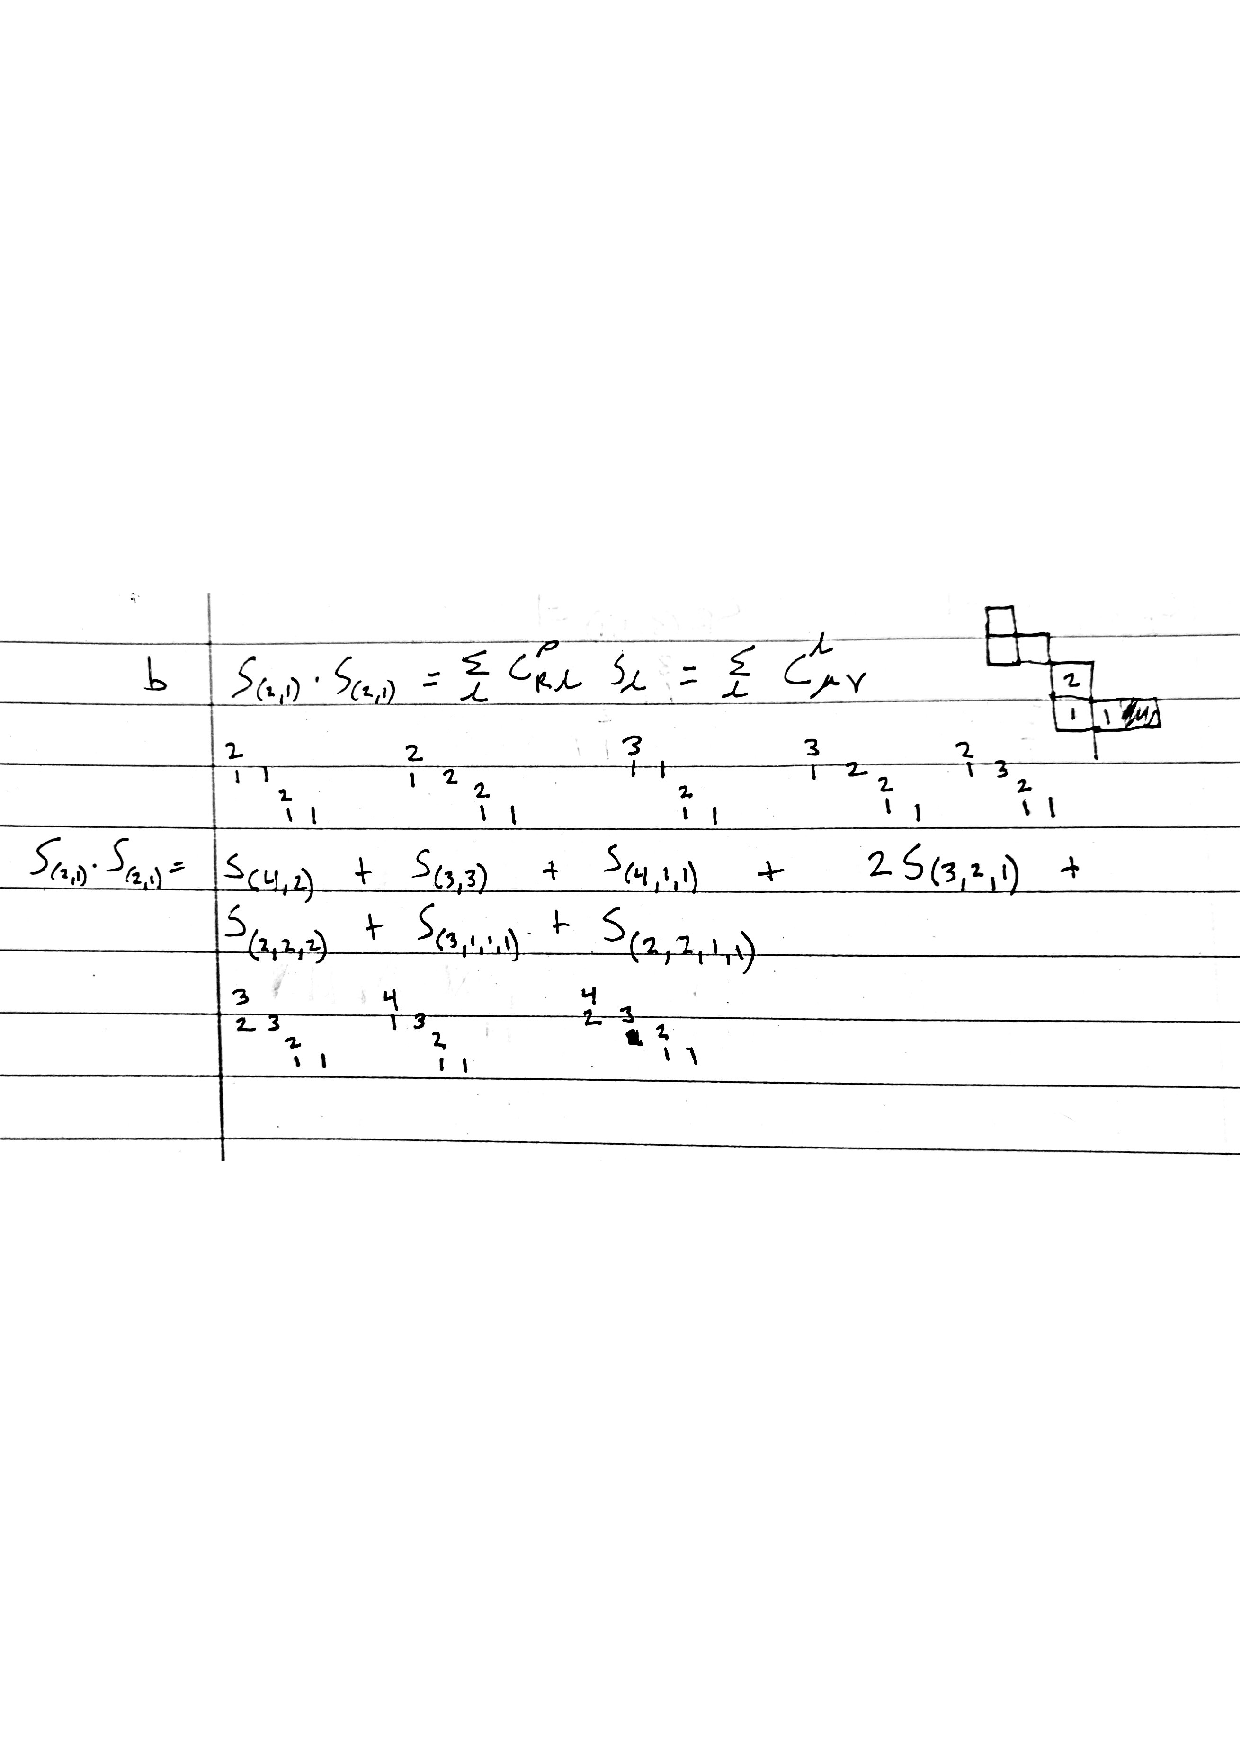
\includegraphics[trim={0 10cm 0 10cm},scale=.6]{pics/hw7fig.pdf}

    where we find that $s_{(2,1)}\cdot s_{(2,1)}=s_{(4,2)}+s_{(3,3)}+s_{(4,1,1)}+2s_{(3,2,1)}+s_{(2,2,2)}+s_{(2,2,1,1)}$

    \item Finally using the inverse frobenious map we know that $\text{Frob}^{-1}(s_{(2,1)}\cdot s_{(2,1)})=V_{(2,1)}\cdot V_{(2,1)}=V_{(4,2)}\oplus V_{(3,3)}\oplus V_{(4,1,1)}\oplus V_{(3,2,1)}\oplus V_{(3,2,1)}\oplus V_{(2,2,2)}\oplus V_{(2,2,1,1)}$.\\
\end{enumerate}


\item[(3)] Let $T=\ytableausetup{smalltableaux}
\ytableaushort{24,31}$ which corresponds the the Garnir polynomial $(x_2-x_3)(x_4-x_1)$. To write this in terms of the basis elements we will first column straighten which gives us the Tablau $T'=\ytableaushort{34,21}$ and that $F_{T}=-F_{T'}$. Then to row straigten we will note that in the first row $2>1$ is out of order meaning we have $A=\ytableausetup{smalltableaux}
\ytableaushort{2,3}$ and $B=\ytableaushort{1}$. The permutation on the elements $1,2,3$ that preserve the column order are $(),(1\;3\;2), (1\;2)$, and so we have that $0=g_{A,B}F_{T'}=F_{T'}+F_{\ytableaushort{24,13}}-F_{\ytableaushort{34,12}}$. meaning we have that $F_T=F_{\ytableaushort{24,13}}-F_{\ytableaushort{34,12}}$.\\

\item[(4)] (not completed for points) I spent a long time thinking about this problem from a categorical perspective. My idea was to use Frobinuous resiprocity, the fact that the induced representation and restriction are adjunct pairs, to decompose the one big inducted representation functor into the composition of other adjuction functors that correspond to outer tensor products. However things got a little messy and i wasn't totally sure how to complete it. I think i understand the idea and with more time im sure it would work.\\  %Let $\lambda$ be a partition of $n$ and consider the representation $\Ind_{S_\lambda}^{S_n}V_{(\lambda_1)}\otimes V_{(\lambda_2)}\otimes\cdots V_{(\lambda_k)}$. Notice that each $V_{(\lambda_i)}$ which is the trivial representation of $S_{\lambda_i}$ a $1$ dimensional subspace and so $V_{(\lambda_1)}\otimes V_{(\lambda_2)}\otimes\cdots V_{(\lambda_k)}\cong 1_{S_\lambda}$ is the trivial representation on $S_\lambda$. Combinatorially we know that $\Ind_{S_\lambda}^{S_n}1_{S_\lambda}$ is isomorphic to the space generated by the cosets of $S_{\lambda}$ which is equivalent to the rearrangements od

%Fix some partition $\lambda$ of $n$ and notice that 
%\begin{tikzcd}[row sep=1cm, column sep=.7cm]
%     \C S_{\lambda_1}\text{-Mod}&\C S_{\lambda_1}\text{-Mod}&&
%    \end{tikzcd}

\item[(5)] Consider the representation of $S_3$ that is the space $V_{(2,1)}\otimes_{inn} V_{(2,1)}=\text{span}((x_2-x_1),(x_3-x_1))\otimes_{inn} \text{span}((y_2-y_1),(y_3-y_1))=\text{span}(v_1,v_2,v_3,v_4)$ where $v_1=(x_2-x_1)(y_2-y_1),v_2=(x_3-x_1)(y_2-y_1),v_3=(x_2-x_1)(y_3-y_1),$ and $v_4=(x_3-x_1)(y_3-y_1)$. In this case also notice that $v_1-v_2=(x_2-x_3)(y_2-y_1), v_2-v_4=(x_3-x_1)(y_2-y_3), v_3-v_4=(x_2-x_3)(y_3-y_1), v_1-v_3=(x_2-x_1)(y_2-y_3), $ and $v_1-v_2-v_3+v_4=(x_2-x_3)(y_2-y_3)$. Now we can consider permutations from each conjugacy class of $S_3$, $(), (1\;2),$ and $(1\;2\;3)$ and consider the matrices that act basis elements that generate the space above. We find that 
$$()\mapsto \begin{pmatrix}1&0&0&0\\0&1&0&0\\0&0&1&0\\0&0&0&1\\\end{pmatrix}\;\;\;\;\;\;\;(1\;2)\mapsto \begin{pmatrix}1&1&1&1\\0&-1&0&-1\\0&0&-1&0\\0&0&0&1\\\end{pmatrix}$$
$$(1\;2\;3)\mapsto \begin{pmatrix}1&1&1&1\\-1&0&-1&0\\-1&-1&0&0\\1&0&0&0\\\end{pmatrix}$$
And looking at the traces we can construct character of this representation $\chi'$

\begin{tabular}{c|ccc}
    $S_3$ & $()$ & $(1\;2)$ & $(1\;2\;3)$\\\hline
    $\chi_{(3)}$ & 1& 1&1  \\
    $\chi_{(2,1)}$ & 2& 0&1\\
    $\chi_{(1,1,1)}$ & 1& -1&1\\
    $\chi'$ & 4& 0&1\\
\end{tabular}

 And from the following table we can determine that $\chi'=\chi_{(1,1,1)}+\chi_{(2,1)}+\chi_{(3)}$ and so $V_{(2,1)}\otimes_{inn} V_{(2,1)}=V_{(1,1,1)}\oplus V_{(2,1)}\oplus V_{(3)}$\\

 \item[(6)] There are $4$ boarder tableau of shape $(3,3,1)$ and content $(3,3,1)$. These are\\\\
 \ytableaushort{1,123,122} \;\;\; where $(-1)^{\text{ht}(\text{strip }1)+\text{ht}(\text{strip }2)+\text{ht}(\text{strip }3)}=-1$\\
 \ytableaushort{3,122,112} \;\;\; where $(-1)^{\text{ht}(\text{strip }1)+\text{ht}(\text{strip }2)+\text{ht}(\text{strip }3)}=1$\\
 \ytableaushort{3,222,111} \;\;\; where $(-1)^{\text{ht}(\text{strip }1)+\text{ht}(\text{strip }2)+\text{ht}(\text{strip }3)}=1$\\
\ytableaushort{2,223,111} \;\;\; where $(-1)^{\text{ht}(\text{strip }1)+\text{ht}(\text{strip }2)+\text{ht}(\text{strip }3)}=-1$,  

And so $\chi_{(3,3,1)}((3,3,1))=0$


\end{itemize}

\end{document}






